
\begin{frame}
\frametitle{Accuracy measures for regression}
\begin{itemize}
\item {\bf Root-mean squared error} for point predictions.
\item {\bf Correlation coefficient} for point predictions.
\item {\bf Log predictive probability} can be used for probabilistic predictions.
\item {\bf Expected loss/risk} for point predictions for decision making.
\end{itemize}
\end{frame}

\begin{frame}
\frametitle{Accuracy measures for binary classification}
\begin{columns}
\column{0.7\textwidth}
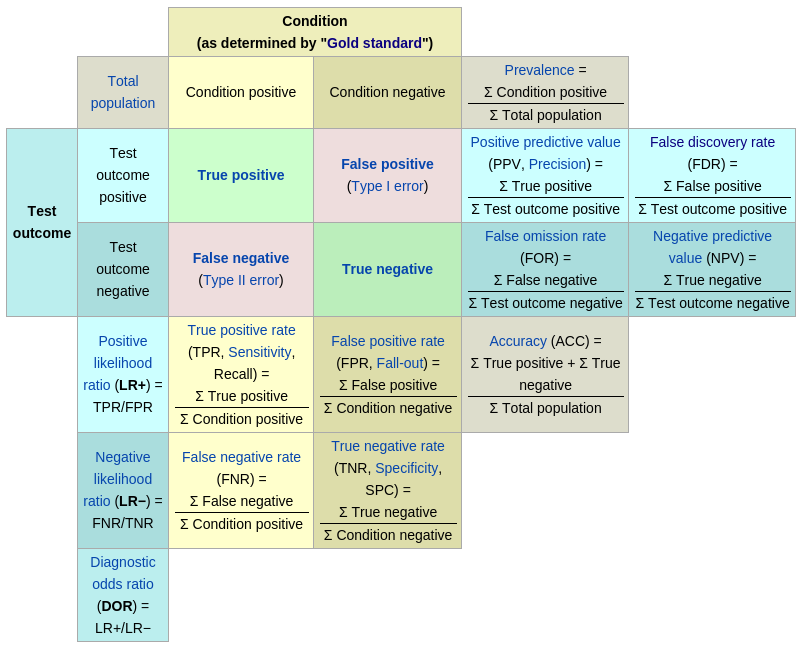
\includegraphics[width=\textwidth]{contingency_table_wikipedia}
%\vspace{0.25cm}
\column{0.3\textwidth}
%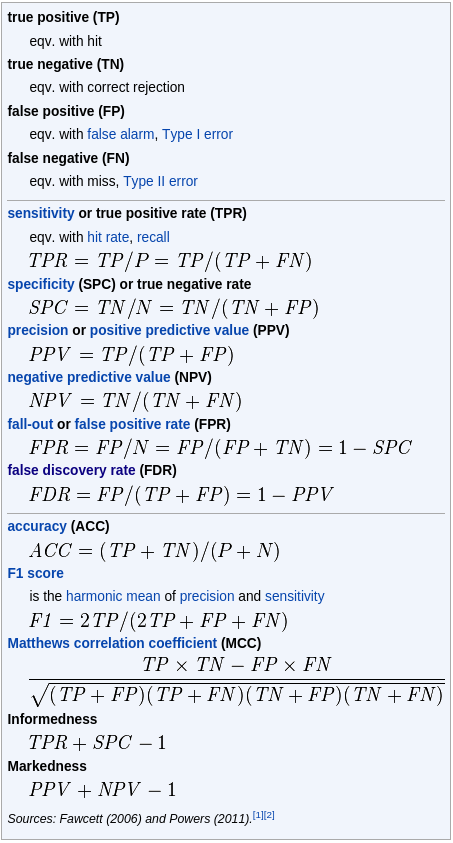
\includegraphics[width=\textwidth]{spec_sens_wikipedia}
\begin{tiny}
Wikipedia contributors, ``Sensitivity and specificity,'' Wikipedia, The Free Encyclopedia, \url{http://en.wikipedia.org/w/index.php?title=Sensitivity\_and\_specificity\&oldid=655245669} (accessed April 9, 2015).\par
\end{tiny}
\end{columns}
\end{frame}

\begin{frame}
\frametitle{Accuracy measures from ROC curve}
\begin{columns}
\column{0.5\textwidth}
The {\bf Receiver operating characteristic} (ROC) curve is a plot of \emph{true-positive rate} (sensitivity) versus \emph{false-positive rate} (1-specificity) over the full range of possible thresholds.\par
\vspace{0.25cm}
The {\bf area under the curve} (AUC) is the integral under the ROC curve.\par
\column{0.5\textwidth}
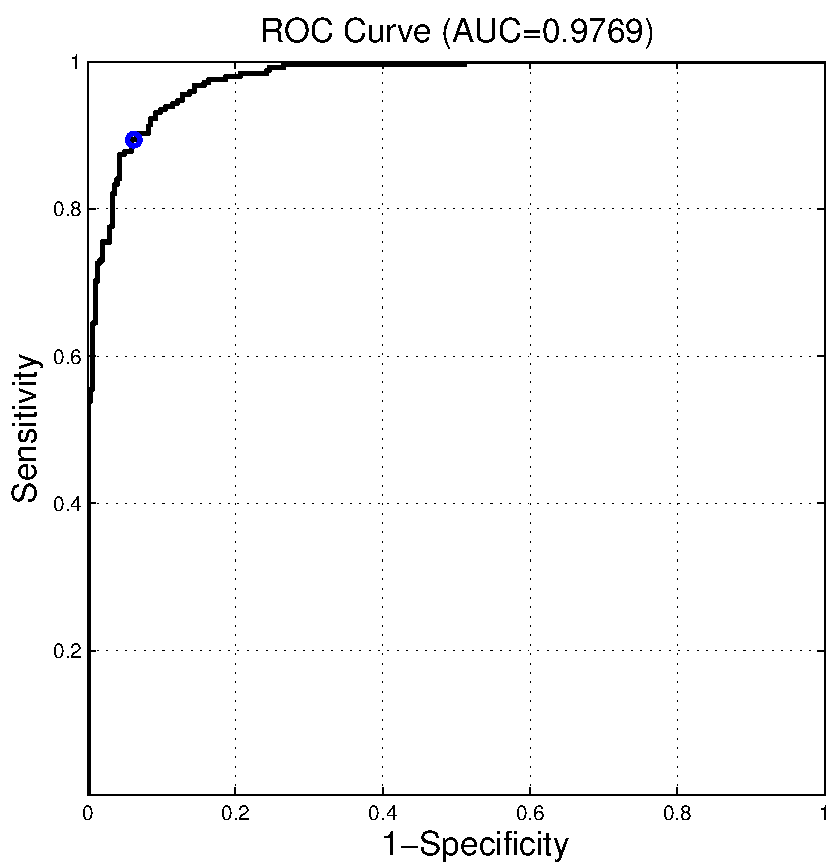
\includegraphics[width=\textwidth]{roc}
\end{columns}
\end{frame}

\begin{frame}
\frametitle{Accuracy measures from precision-recall curve}
\begin{columns}
\column{0.5\textwidth}
The {\bf precision-recall} (PR) curve is a plot of \emph{relevance} (precision) versus \emph{completeness} (recall) over the full range of possible thresholds.\par
\vspace{0.25cm}
The $F_1$ score is the harmonic mean of precision and recall for a given threshold. The AUC can also be used.\par
\column{0.5\textwidth}
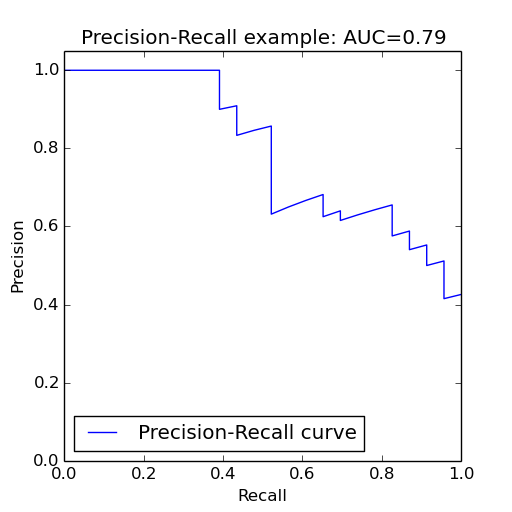
\includegraphics[width=\textwidth]{sklearn_material/PR}
\end{columns}
\end{frame}


\begin{frame}
\frametitle{Log predictive probability}
Some data are more easily classified than others.\par
Probabilistic classifiers provide a level of confidence for each prediction.
\begin{align*}
p(y_*|{\bf x}_*,{\bf y},{\bf X},\theta)
\end{align*}
Quality of predictions can be assessed using the {\bf test log predictive probability}:
\begin{align*}
\tfrac{1}{m}\sum_{i=1}^m \log_2 p(y_{*i}\!=\!t_i|{\bf x}_{*i},{\bf y},{\bf X},\theta)
\end{align*}
After subtracting the baseline measure, this shows the average bits of information given by the model.\par
\vspace{0.25cm}
\begin{tiny}
Rasmussen \& Williams. ``Gaussian Processes for Machine Learning'', MIT Press (2006).\par
\url{http://www.gaussianprocess.org/gpml/}\par
\end{tiny}
\end{frame}

